\chapter{Concepts}

\section{Compile Time Generated Database}
\begin{figure}[h!]
    \centering
    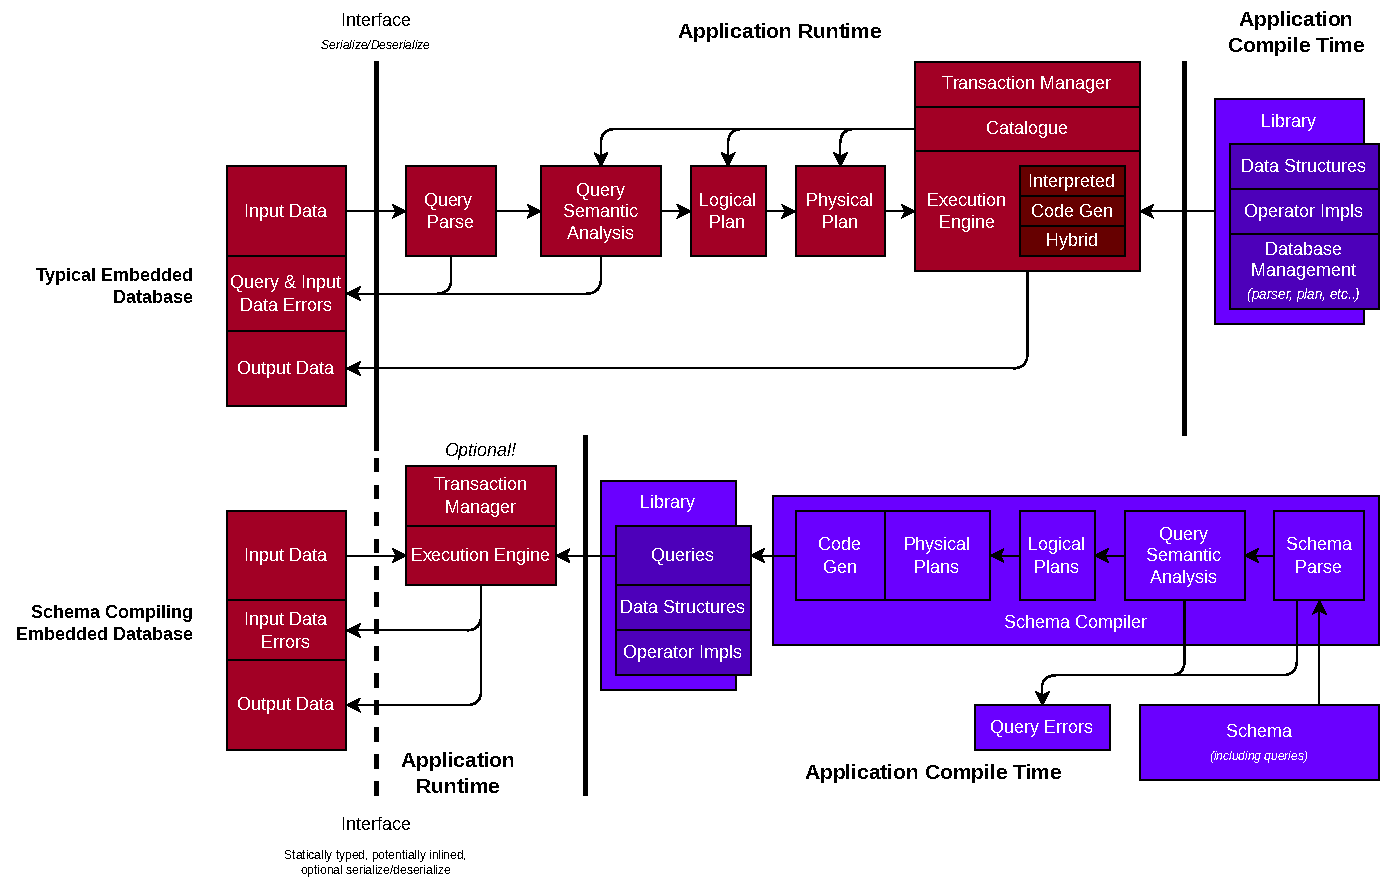
\includegraphics[width=\textwidth]{concepts/_diagrams/query_lifespan.pdf}
    \caption{Comparison between schema compilation and typical embedded databases}
\end{figure}
\noindent
By requiring a static schema, and known parameterized-queries at application compile time, rather than at runtime, we gain the following benefits:
\begin{itemize}
    \setlength\itemsep{0em}
    \item Logical optimisations on both queries and tables (i.e. data structure selection, index selection) can occur, with the entire context of all possible queries.
    \item Errors in queries (that are not dependent on the input data, e.g type errors, invalid table access) can be reported at application compile time.
    \item Time to query parse, analyse and plan is entirely eliminated, this allows more expensive query optimisation to be performed with no cost to the query's execution time.
          This is beneficial for code generation, which can provide performance benefits, at a large upfront cost (for example degrading performance of small queries for HIQUE\cite{HIQUEPaper}, and the motivation for generating code at the LLVM IR level (rather than C++) for hyper\cite{HyperCodegen}.)
\end{itemize}
\begin{quote}
    \textit{"The parsing of SQL statements is a significant consumer of CPU cycles in any SQL database engine. On-going efforts to optimize SQLite have caused the developers to spend a lot of time tweaking Lemon to generate faster parsers."}
    \\ \vspace{0.5cm}
    \hfill -- \textit{SQLite Website\cite{SQLiteLemonParser}}
\end{quote}

As the schema is compiled alongside the application, a greater level of integration with the application is possible.
\begin{itemize}
    \setlength\itemsep{0em}
    \item One of the major benefits touted for embedded databases such as SQlite, DuckDB and monetdb/e is that they provide language
          agnostic interfaces, allowing them to be portable to embed in applications of many different languages.
    \item Portability comes at the cost of providing a uniform interface across different languages (SQL strings). Which thus cannot take advantage of semantics specific to the host language (for example move semantics in C++ \& Rust, or lifetime bound references in Rust).
\end{itemize}
By forgoing portability and generating an interface in the host language, we can take advantage of such semantics, 
and allow for further optimisation (e.g. inlining queries, constant propagation into queries).
\\
\\ It also makes it possible to embed complex logic into the database.
\begin{minted}{rust}
fn my_complex_logic(borrowed_string: &str) -> bool { /* ... */ }

const SOME_LIMIT: usize = /* ... */;

emql!{
    table some_data { string_field: String, const_string_field: &'static str, /* ... */ }

    // For example a query defined in emQL, using user types and functions, with relational algebra
    query some_query(foo: crate::UserDefinedType, bar: &'qy (String, usize)) {
        use some_data  // scan table
            |> filter(crate::my_complex_logic(string_field) || bar.1 < crate::SOME_LIMIT)
            |> // ... do some aggregations: groupby, join, map, etc.
            ~> return;
    }
    // ...
}
\end{minted}

\subsection{Logical Optimisation}

\subsubsection{No Update - Immutable Values}
\label{sec:mut_opt}
When values are not updated, can be shared when accessed from the database, without needing to copy, 
with the caveat that the data returned needs to be wrapped in some safe reference type. There are several options for this:
\begin{itemize}
    \setlength\itemsep{0em}
    \item Borrows (pointer qualified by the lifetime of the database) are the simplest, but require pointer stability (the data cannot be freed or moved while the reference is valid).
    \item Reference counting is more flexible, but requires a more complex implementation (including reference counts).
    \item With an extra level of indirection, reference counting can be applied to mutable values (always allocate a new tuple on update, requires copying over unchanged values from the old allocation).
\end{itemize}
The advantage of avoiding copies of immutable data is directly tied to the cost of the copy. For small values (i.e. 8 byte and less) 
this is irrelevant as it is equal or less cost than moving a pointer (8 bytes on 64 bit systems).

\subsubsection{No Delete - Append Only Tables}
\label{sec:app_opt}
Keys to data structures that allow deletions require checks that append only data structures do not.
\begin{enumerate}
    \setlength\itemsep{0em}
    \item If the database supports queries returning stable row references / \mintinline{SQL}{rowid}, if there are no deletions then no additional data is required other than an index (which can be used to lookup the table), versus requiring a generation count and generation check for tables supporting deletion. DuckDB supports returning unsatble \mintinline{SQL}{rowid} (row ids for deleted rows may be later reused)\cite{DuckDBRowid}, SQLite supports stable \mintinline{SQL}{rowid} if the table has an \mintinline{SQL}{INTEGER PRIMARY KEY} for rowid tables\cite{SQLiteRowIDTables}.   
    \item If the database is using immutable value optimisation (\ref{sec:mut_opt}), the lack of deletion operations can inform the choice of data structure \& hence the type of reference. 
    \item Negligable cost of checking for free slots in a table can be removed, only need to append.
\end{enumerate}


\subsubsection{No Insert - Static Data}
If some data is required, but never updated, inserted or deleted. It can be used for optimisations:
\begin{itemize}
    \item Given a known set of values, \textit{perfect hashing} can be used to accelerate aggregations and joins.
\end{itemize} 
\begin{minted}{rust}
table countries {
    name: String, // country names immutable, and no new countries added 
    population: usize, // other fields can be updated
    // ...
} // with some static data at the start
\end{minted}

\subsubsection{Limited Table Sizes}
For some schemas a bound on the maximum size of a table is known at compile time. This can be used to allocate a fixed size table.
\begin{itemize}
    \setlength\itemsep{0em}
    \item This can be used to eliminate the need to allocate (e.g. extend vectors, or allocate new blocks). This can be a requirement for memory constrained systems, such as in embedded programming.
    \item Fixed size buffers have both fast lookup, and pointer stability.
\end{itemize}

\subsubsection{Incremental View Maintenance (IVM)}
\begin{tcbraster}[raster columns=2,raster equal height]
    \begin{definitionbox}{Views}
        \centerline{\textbf{Recompute on Access}}
        \begin{minted}{SQL}
CREATE VIEW my_view AS SELECT * FROM ..;            
        \end{minted}
        An alias for a query, typically a \mintinline{SQL}{SELECT} statement, that can be queried like a table. The view's query is used each time it is accessed.\cite{Postgres16Docs}
    \end{definitionbox}
    \begin{definitionbox}{Materialized Views}
        \centerline{\textbf{Recompute on Change}}
        Views with results cached. The contained query is only recomputed after a change in the data the query relies on. Beneficial for expensive queries that are frequently accessed and depend on infrequently changing data.
    \end{definitionbox}
\end{tcbraster}
\noindent
The aim of incremental view maintenance is to support views on data that \textbf{Never Recompute} in their entirety, but instead can updated \textit{incrementally} using changes applied to source relations.
\begin{figure}[h!]
    \centering
    \includegraphics[width=\textwidth]{concepts/_diagrams/ivm.pdf}
    \caption{Incremental View Maintenance as a Calculus}
\end{figure}
\noindent
The cost reduction from recomputing operators to recomputing the deltas of operators can also be applied recursively. 
DBToaster (\ref{sec:db_toaster}) generates IVM C++ code for a schema of select queries and input streams. As a 
result it cannot support complex mutation:
\begin{minted}{SQL}
UPDATE .. WHERE ( COMPLEX EXPRESSION )
\end{minted}
\noindent
There is no fundamental barrier to an IVM system supporting this.
\\
\\ IVM performance can benefit from restrictions of the operations that can occur on tables.
\subsection{Physical Optimisation}
\subsubsection{Profile Guided Optimisation}
Given the queries are known, they can be instrumented to collect statistics at runtime, for use in subsequent compilations.
\begin{itemize}
    \setlength\itemsep{0em}
    \item These features are already available for many languages, by compiling the schema to a language that supports profile-guided optimisation this feature is atained for free.
\end{itemize}

\subsubsection{Ownership Transfer}
\label{sec:ownership_transfer}
Given the host language supports move-semantics, queries can \textit{move} arguments. Moving owning objects only requires a copy of the data structure, and not a deep copy of data (i.e. heap allocated) owned by it.
\begin{itemize}
    \setlength\itemsep{0em}
    \item Ensuring the data is not accidentally mutated after ownership is given to the database, or mitigating ease of doing this is a memory safety requirement for the database.
\end{itemize}

\subsubsection{User Defined Types}
Rather than enforcing users to serialize data for use in the database, or rely on general implementations for copying, hashing \& 
\begin{itemize}
    \setlength\itemsep{0em}
    \item Removal of serialization can benefit performance, particularly when combined with ownership transfer\ref{sec:ownership_transfer}.
\end{itemize}